\documentclass[conference]{IEEEtran}

\usepackage{cite}
\usepackage{amsmath,amssymb,amsfonts}
\usepackage{graphicx}
\usepackage{textcomp}
\usepackage{xcolor}
\usepackage{hyperref}
\usepackage{booktabs}
\usepackage{listings}

\hypersetup{
    colorlinks=true,
    linkcolor=blue,
    citecolor=blue,
    urlcolor=blue,
}

\renewcommand{\ttdefault}{cmtt}

\lstdefinelanguage{Solidity}{
    keywords={pragma, solidity, contract, abstract, function, modifier, require, bool, address, uint256, internal, external, public, payable, returns, if, else, revert, emit, msg, this, true, false, using, for},
    morecomment=[l]{//},
    morecomment=[s]{/*}{*/},
    morestring=[b]",
    sensitive=true,
}

\lstset{
    basicstyle=\ttfamily\footnotesize,
    breaklines=true,
    frame=single,
    language=Solidity,
    numbers=left,
    numberstyle=\tiny,
    keywordstyle=\bfseries,
    commentstyle=\itshape,
    tabsize=4,
    columns=flexible,
}

\setlength{\textfloatsep}{6pt plus 1pt minus 1pt}
\setlength{\floatsep}{6pt plus 1pt minus 1pt}

\begin{document}

\title{From Findings to Verifiable Remediation Artifacts: A Smart Contract Security Pipeline}

\author{
\IEEEauthorblockN{Fernando Boiero, Sebasti\'an Norberto Mussetta, and Norberto Gaspar Cena}
\IEEEauthorblockA{
\textit{Universidad Tecnol\'ogica Nacional (UTN)}\\
\textit{Facultad Regional Villa Mar\'ia}\\
Villa Mar\'ia, C\'ordoba, Argentina\\
\{fboiero, smussetta, ngcena\}@frvm.utn.edu.ar}
}

\maketitle

\begin{abstract}
Detection tools usually stop at the finding: they identify a vulnerable function, but the patch, regression test, and audit evidence remain manual work. This paper evaluates how far an automated pipeline can move from a finding to inspectable remediation artifacts without hiding residual failures. MIESC takes normalized Solidity findings, emits nearly self-contained patch candidates, generates Foundry exploit tests, creates formal-specification stubs, and maps findings to compliance controls. The corpus-scale evaluation targets patch generation; tests, specifications, and compliance mappings are demonstrated on a single illustrative contract. On SmartBugs-curated (143 contracts), the v2 remediation baseline patches 123 contracts, and all 123 patches compile standalone. The MIESC re-scan reports fewer HIGH/CRITICAL findings for 88 of them, and 121 satisfy a bounded no-regression criterion. Under independent Slither validation, 70 patched contracts are free of HIGH findings (57\%; 95\% Wilson CI [48\%, 65\%]). A pre-patch Slither baseline adds independent evidence. Slither's reentrancy detector fires on 28 of 29 analyzable reentrancy contracts before patching and on none after. Among the 121 analyzable patched contracts, those free of HIGH findings rise from 35 to 69 (exact McNemar $p<10^{-9}$), and nearly all remaining HIGH alerts predate the patch. The artifacts are verifiable in that each can be re-checked independently; the repairs are not proven correct. The pipeline runs locally without API calls and automates the generation of repair candidates for human review, not correct automatic repair. Scripts and per-claim artifacts are released; MIESC is available under AGPL-3.0.
\end{abstract}

\begin{IEEEkeywords}
smart contracts, automated program repair, exploit testing, formal verification, security compliance, defense-in-depth
\end{IEEEkeywords}

% ===========================================================================
\section{Introduction}
% ===========================================================================

The smart contract security ecosystem has invested heavily in \emph{detection}---static analyzers~\cite{feist2019slither}, fuzzers~\cite{grieco2020echidna}, symbolic executors~\cite{mueller2018smashing}, and more recently auditors based on large language models (LLMs)~\cite{sun2024gptscan}---but comparatively little in what happens \emph{after} a vulnerability is found. In practice, the workflow looks like this:

\begin{enumerate}
    \item A tool reports: ``Reentrancy in \texttt{withdraw()} (HIGH).''
    \item A developer manually writes a patch (add \texttt{nonReentrant}).
    \item The developer manually writes a test checking the intended fix path.
    \item The developer manually maps the finding to compliance requirements.
    \item The developer manually writes the audit report.
\end{enumerate}

Steps 2--5 require security expertise that many development teams lack. This paper evaluates the remediation pipeline of MIESC (Multi-layer Intelligent Evaluation for Smart Contracts), which exposes the workflow through composable commands:

\begin{verbatim}
miesc scan contract.sol -o results.json
miesc fix results.json \
  -c contract.sol -o fixed.sol
miesc test-gen results.json -c contract.sol
miesc compliance results.json --standard mica
miesc report results.json -t premium -f pdf
\end{verbatim}

We evaluate patch quality on the SmartBugs-curated corpus (143 contracts, 10 vulnerability categories), trace the artifact pipeline on an illustrative vulnerable contract, and compare against five prior automated repair tools. Throughout the paper, \emph{verifiable} refers to the artifacts: each patch, test, specification, and compliance mapping can be re-checked independently. It does not mean that the repairs are proven correct. Likewise, we distinguish the automated \emph{generation of repair candidates}, which is what MIESC provides, from \emph{correct automatic repair}, which our results do not establish. The evidence behind each contribution differs, and we state it explicitly:

\begin{enumerate}
    \item \textbf{Nearly self-contained patch-candidate generation} (\texttt{miesc fix}) --- \emph{evaluated at corpus scale}. Text-level Solidity patch candidates that avoid adding external dependencies (except a SafeMath directive for pre-0.8 arithmetic). Of the 123 contracts patched under the v2 baseline, 57\% (70) are free of HIGH findings under independent Slither validation, the most conservative metric. All 123 patches compile standalone, 72\% reduce the HIGH/CRITICAL count on re-scan, and 98\% satisfy a bounded no-regression criterion. We foreground the external metric because re-scanning with the detecting pipeline is circular.
    \item \textbf{Exploit test generation} (\texttt{miesc test-gen}) --- \emph{demonstrated on one illustrative contract}. Foundry test templates designed to exercise the exploit path on the vulnerable contract and to check that the patched version blocks it; on the illustrative contract, 2 of the 6 tests discriminate between the two versions.
    \item \textbf{Formal specification generation} (\texttt{miesc specs}) --- \emph{demonstrated on one illustrative contract}. Certora Verification Language (CVL) rules, Scribble annotations, and SMTChecker assertions generated from findings.
    \item \textbf{Compliance mapping} (\texttt{miesc compliance}) --- \emph{demonstrated on one illustrative contract}. Rule-based mapping to 12 standard and taxonomy profiles (e.g., ISO~27001, the NIST Cybersecurity Framework (CSF), OWASP, the EU Markets in Crypto-Assets Regulation (MiCA) and Digital Operational Resilience Act (DORA), and the CWE and SWC weakness taxonomies).
    \item \textbf{Pipeline integration and comparison}: a feature-level comparison against SCRepair, sGuard, Elysium, ACFIX, and SCPatcher, showing which remediation artifacts MIESC emits beyond repair-only baselines.
\end{enumerate}

The contribution is therefore one of pipeline integration rather than a new standalone repair technique. Unlike prior repair tools that stop at the patch, MIESC emits patches, exploit tests, formal-specification stubs, and compliance mappings as inspectable artifacts from a single pipeline. From a technology-transfer standpoint, it targets the practical gap development teams face after detection---turning a finding into a reviewable patch, test, and audit artifact inside existing continuous integration and delivery (CI/CD) workflows.

Our evaluation yields three main findings:
\begin{itemize}
    \item \textbf{Nearly dependency-free patches remove the compilation bottleneck.} Inlining guards instead of importing libraries (only a pre-0.8 SafeMath directive remains), together with a scan-filtered denominator, takes standalone compilation from 51 failures in 141 patches (v1) to none in 123 (v2).
    \item \textbf{Slither's reentrancy detector falls silent on patched reentrancy contracts.} Running Slither on the original and the patched files, its reentrancy detector fires on 28 of 29 analyzable reentrancy contracts before patching and on none after. Over all 121 analyzable patched contracts, those free of HIGH findings rise from 35 to 69 and HIGH contract--detector pairs fall from 141 to 60. Detector silence is evidence, not proof, of a correct repair, and unchecked low-level calls have no Slither HIGH detector to confirm them.
    \item \textbf{What remains is mostly untargeted, pre-existing issues.} In 50 of the 52 analyzable contracts that are not clean after patching, every remaining HIGH detector was already present before patching (chiefly array-length control, weak randomness and state shadowing); 2 patches introduce a new HIGH alert. Extending the patch templates to these classes is the next lever.
\end{itemize}

% ===========================================================================
\section{Related Work}
% ===========================================================================

\subsection{Automated Program Repair for Smart Contracts}

SCRepair~\cite{screpair2020} uses genetic programming to mutate Solidity source code until tests pass, but requires pre-existing test suites. sGuard~\cite{nguyen2021sguard} inserts runtime checks (reentrancy locks, integer overflow guards) at near-100\% compilation but does not generate tests to verify the fix. Elysium~\cite{elysium2022} patches at the bytecode level and reports correctly patching at least 30\% more contracts than existing tools, but covers 7 vulnerability types. ACFIX~\cite{acfix2024} uses LLMs guided by mined role-based access control (RBAC) practices and repairs 94.9\% of 118 access-control vulnerabilities, but targets a single vulnerability class. SCPatcher~\cite{scpatcher2025} applies LLMs with retrieval-augmented generation (RAG) to general-purpose patching, reporting 81.5\% fix rate and 91\% compilation.

MIESC differs in three ways: (1)~patch candidates are \emph{self-contained} in the sense that they avoid new library imports (the pre-0.8 SafeMath directive is the exception), (2)~exploit tests are generated alongside patches to check the vulnerable and patched paths, and (3)~the pipeline extends beyond patching to formal specifications and compliance mapping. Section~\ref{sec:comparison} provides a detailed feature comparison.

\subsection{Test Generation for Smart Contracts}

Foundry~\cite{foundry2025} and Echidna~\cite{grieco2020echidna} provide fuzzing and property-based testing frameworks, but require developers to write test properties manually. Harvey~\cite{harvey2020} generates high-coverage test inputs but not exploit-specific test cases.

MIESC's \texttt{test-gen} command generates vulnerability-specific exploit tests: a reentrancy finding produces a test with an attacker contract that re-enters the victim, while a selfdestruct finding produces an unauthorized-caller test. The generated artifacts serve two roles: exploit-confirmation tests are designed to exercise the vulnerable behavior on the original contract, and fixed-version regression tests check that the same path is blocked after patching.

\subsection{Compliance Automation}

In the repair tools surveyed in this paper, compliance mapping is outside the reported scope. Mapping findings to standards such as ISO~27001, MiCA, and NIST CSF is typically performed manually by auditors during report writing. MIESC automates this with a rule-based mapper covering 12 standard and taxonomy profiles.

\subsection{LLM-Assisted Security Analysis}

GPTScan~\cite{sun2024gptscan} combines GPT-4 with program analysis for logic vulnerability detection but produces no patches. EVMbench~\cite{evmbench2026} evaluates LLM agents on real audit findings in detect, patch and exploit modes; its patch mode scores agent-written fixes against the benchmark's exploit tests, whereas MIESC emits rule-based patch candidates together with their own tests, specifications and compliance mapping. The SmartBugs framework~\cite{smartbugs2023} provides execution infrastructure for tool evaluation but includes no patching capabilities. MIESC builds on these detection advances by extending the pipeline beyond detection into actionable remediation artifacts.

% ===========================================================================
\section{Pipeline Architecture}
% ===========================================================================

The remediation pipeline consists of five stages, each consuming the output of the previous stage (Figure~\ref{fig:pipeline}).

\begin{figure}[htbp]
\centering
\footnotesize
\setlength{\fboxsep}{2pt}
\setlength{\fboxrule}{0.3pt}
\begin{tabular}{c}
\fbox{{\scriptsize \textbf{Stage 1}: \texttt{miesc scan} $\rightarrow$ findings.json}} \\[2pt]
$\downarrow$ \\[1pt]
\fbox{{\scriptsize \textbf{Stage 2}: \texttt{miesc fix} $\rightarrow$ contract.fixed.sol}} \\[2pt]
$\downarrow$ \\[1pt]
\fbox{{\scriptsize \textbf{Stage 3}: \texttt{miesc test-gen} $\rightarrow$ test/*.t.sol}} \\[2pt]
$\downarrow$ \\[1pt]
\fbox{{\scriptsize \textbf{Stage 4}: \texttt{miesc specs} + \texttt{miesc verify}}} \\[2pt]
$\downarrow$ \\[1pt]
\fbox{{\scriptsize \textbf{Stage 5}: \texttt{miesc compliance} + \texttt{miesc report}}}
\end{tabular}
\caption{MIESC remediation pipeline. Each stage consumes the output of the previous stage, producing a progressively more complete security artifact.}
\label{fig:pipeline}
\end{figure}

\subsection{Stage 1: Detection}

Detection is described in our companion paper~\cite{boiero2025miesc} and is out of scope here; this paper consumes its output. The scanner emits a normalized JSON with findings, severity, location, confidence, canonical category, and remediation fields consumed by the patcher.

\subsection{Stage 2: Patch Generation}

\texttt{miesc fix} applies text-level patches to the original Solidity source. The patcher operates on the finding's type and function location:

\begin{itemize}
    \item \textbf{Reentrancy}: inserts \texttt{nonReentrant} modifier. If OpenZeppelin is not detected, inlines a self-contained \texttt{MiescReentrancyGuard} contract (9 lines).
    \item \textbf{Access control / selfdestruct}: inserts \texttt{onlyOwner} modifier. If no modifier is defined, inlines a 5-line \texttt{onlyOwner} modifier using the existing \texttt{owner} state variable.
    \item \textbf{Unchecked calls}: wraps value-bearing low-level calls in \texttt{require(success)}.
    \item \textbf{Arithmetic (pre-0.8)}: inserts \texttt{using SafeMath for uint256}; unlike the other fixes, this one requires a SafeMath library in the compilation unit, which the 4 patched arithmetic contracts provide.
\end{itemize}

A deduplication step tracks \texttt{(function, fix\_category)} pairs to avoid applying the same fix twice when multiple findings target the same function (e.g., \texttt{suicidal} and \texttt{selfdestruct-identifier} both targeting \texttt{destroy()}).

Function name inference: when findings lack an explicit function name (common for LLM-based detections), the patcher infers the nearest function declaration above the reported line number.

\subsubsection{Patch Example: Reentrancy Guard Injection}

Listing~\ref{lst:before} shows a vulnerable withdrawal function. The external call on line~3 occurs \emph{before} the state update on line~5, enabling a classic reentrancy attack. Listing~\ref{lst:after} shows MIESC's patched version: the inline \texttt{MiescReentrancyGuard} (lines~1--9) provides a self-contained mutex that compiles without external dependencies, while the \texttt{nonReentrant} modifier on line~14 blocks re-entry. This inline approach avoids requiring OpenZeppelin imports, which is critical for standalone compilation of legacy contracts.

\begin{lstlisting}[caption={Vulnerable: external call before state update},label={lst:before},float=htbp]
function withdraw(uint256 amount) external {
    require(balances[msg.sender] >= amount);
    (bool ok,) = msg.sender.call{value: amount}("");
    require(ok);
    balances[msg.sender] -= amount;
}
\end{lstlisting}

\begin{lstlisting}[caption={Patched: inline reentrancy guard injected by MIESC},label={lst:after},float=htbp]
contract MiescReentrancyGuard {
    bool internal _locked;
    modifier nonReentrant() {
        require(!_locked, "ReentrancyGuard: reentrant");
        _locked = true;
        _;
        _locked = false;
    }
}

contract Vault is MiescReentrancyGuard {
    // ...
    function withdraw(uint256 amount)
        external nonReentrant
    {
        require(balances[msg.sender] >= amount);
        (bool ok,) = msg.sender.call{value: amount}("");
        require(ok);
        balances[msg.sender] -= amount;
    }
}
\end{lstlisting}

The guard uses only basic state and modifier syntax, so it compiles with every compiler the corpus required (solc 0.4.24--0.5.17); the surrounding example uses 0.8 syntax for readability, and compatibility with 0.6--0.8 code was not evaluated on the corpus. For contracts already inheriting from OpenZeppelin's \texttt{ReentrancyGuard}, the patcher detects the existing import and adds only the modifier annotation.

\subsection{Stage 3: Exploit Test Generation}

\texttt{miesc test-gen} generates one Foundry test file per finding. Each test is designed with a dual-assertion property:

\begin{itemize}
    \item \textbf{Against vulnerable contract}: the test should \emph{demonstrate} the exploit (fail assertion or trigger unexpected behavior).
    \item \textbf{Against fixed contract}: the test should \emph{pass} (exploit is blocked by the patch).
\end{itemize}

Templates exist for reentrancy (deploys attacker contract with re-entrant \texttt{receive()}), access control and selfdestruct (\texttt{vm.prank} + \texttt{vm.expectRevert} for a non-owner caller), unchecked calls (reverting receiver contract), and a generic state-initialization check.

\subsection{Stage 4: Formal Specification}

\texttt{miesc specs} generates executable specifications from findings:
\begin{itemize}
    \item \textbf{Certora CVL}: a \texttt{noReentrancy} rule targeting the vulnerable function.
    \item \textbf{Scribble}: inline annotations (\texttt{/// \#if\_succeeds ...}).
    \item \textbf{SMTChecker}: \texttt{assert()} statements encoding the post-patch property (e.g., balance invariants, checked call results).
\end{itemize}

\texttt{miesc verify} executes specifications against available provers (Certora, Halmos, solc SMTChecker).

\subsection{Stage 5: Compliance and Reporting}

\texttt{miesc compliance} maps each finding to applicable standards using a rule-based mapper with 12 standard and taxonomy profiles. \texttt{miesc report} generates audit reports in HTML, PDF, Markdown, or SARIF (Static Analysis Results Interchange Format) with CVSS scores, remediation roadmaps, and executive summaries.

% ===========================================================================
\section{Evaluation}
% ===========================================================================

\subsection{Experimental Setup}
\label{sec:setup}

We evaluate the remediation stage on the SmartBugs-curated corpus~\cite{ferreira2020smartbugs}: 143 contracts spanning 10 vulnerability categories (reentrancy, access control, unchecked low-level calls, arithmetic, denial of service, front running, short addresses, time manipulation, bad randomness, and other). The remediation metrics and a per-claim trace are generated by the benchmark scripts in the repository. The v2 baseline also runs opt-in Slither validation on patched contracts that compile, recording external HIGH findings separately from the internal MIESC re-scan. Derived artifacts further summarize patch quality by transformation class and standalone compilation failures by category.

\textbf{Metric definitions.} \emph{Fix applied} means the patcher produced a modified source file for at least one fixable HIGH/CRITICAL finding. \emph{Standalone compilation} means the patched file compiles without restoring the original project dependency tree. \emph{Vulnerability eliminated} means that a MIESC re-scan of the patched contract reports fewer HIGH/CRITICAL findings than the scan of the original; it is a count-based criterion, not a check that the specific targeted finding disappeared. \emph{No regression} is a bounded re-scan criterion: the patched contract does not increase the finding count by more than one extra finding (tolerance$=$1) under the same scanner; it is not a proof of full functional equivalence. Under the strict criterion (tolerance$=$0, no additional findings permitted) the rate is 115/123 (93\%); the reported 98\% (121/123) admits the single extra guard-related finding that patch insertion commonly introduces. The full tolerance sensitivity curve (0--10) is released with the artifacts. \emph{External clean-HIGH} means a separate Slither validation run over patched contracts that compile reports no HIGH findings. For the \emph{pre-patch baseline}, we run the same Slither version (0.11.6, as pinned in the repository) with the same compiler per contract on the original files; because one detector proved nondeterministic, each original is analyzed ten times and a detector counts as present if any run reports it. Slither's parser crashes on two original reentrancy contracts (a tuple-assignment construct), although both compile; baseline comparisons therefore cover 121 of the 123 patched contracts. For proportions we report 95\% Wilson score intervals, which remain well behaved for the small per-category denominators.

\textbf{Baselines v1 and v2.} Two patcher versions appear in this paper. The v1 run patched 141 contracts, and 51 of those patches failed standalone compilation (42 undefined-symbol and 9 other compiler errors), mostly because guards referenced library symbols that the standalone file did not declare. The v2 patcher makes two changes: (i)~it injects \emph{inline} guards and modifiers (e.g., \texttt{MiescReentrancyGuard}) instead of relying on imported libraries, and (ii)~it computes the denominator from the \emph{current} scan, excluding contracts with no current HIGH/CRITICAL finding (18) or empty scan output (2). All results below refer to v2 unless stated otherwise; v1 figures are given only to explain the change. Table~\ref{tab:denominators} reconciles the denominators used across sections.

\begin{table}[htbp]
\caption{Denominator Reconciliation}
\label{tab:denominators}
\centering
\footnotesize
\setlength{\tabcolsep}{3pt}
\begin{tabular}{@{}rp{0.74\columnwidth}@{}}
\toprule
\textbf{$n$} & \textbf{Population and where it is used} \\
\midrule
143 & SmartBugs-curated corpus (all contracts) \\
142 & Original (unpatched) files that compile standalone (validity audit) \\
141 & Contracts patched by the v1 patcher (historical comparison only) \\
123 & v2 patched contracts: $143 - 18$ no-HIGH $- 2$ empty-scan; denominator of all v2 rates \\
121 & Patched contracts with a valid pre-patch Slither run (Table~\ref{tab:prepost}) \\
29 & Of these, reentrancy contracts \\
\bottomrule
\end{tabular}
\end{table}

As an illustrative example, we also trace the full pipeline end-to-end on a single test contract (\texttt{AuditTarget.sol}) containing 5 intentional vulnerabilities (reentrancy, missing access control, unprotected selfdestruct, missing zero-address check, and centralized emergency withdrawal). This end-to-end trace is an illustrative walkthrough: the per-stage counts in Table~\ref{tab:tests} and Section~\ref{sec:e2e} describe this single contract and are not corpus-wide claims.

\textbf{Environment}: macOS ARM64 (Apple Silicon), 48\,GB RAM, Foundry v1.3.5. Corpus contracts are compiled with the solc version selected from their pragma (0.4.24--0.5.17); the illustrative contract uses Solidity 0.8.20. The remediation evaluation was re-run after the final detection profile of the companion paper~\cite{boiero2025miesc}; remediation and detection metrics are kept as separate reproducibility artifacts.

\subsection{Stage 2: Patch Quality}

\begin{table}[htbp]
\caption{Aggregate Patch Generation Results (v2; 143 contracts, 123 patched)}
\label{tab:fix}
\centering
\begin{tabular}{@{}lccc@{}}
\toprule
\textbf{Metric} & \textbf{Count} & \textbf{Rate} & \textbf{95\% CI} \\
\midrule
Fix applied (current scan) & 123/143 & 86\% & [79, 91] \\
Compilation (standalone) & 123/123 & 100\% & [97, 100] \\
Vuln.\ eliminated (fewer HIGH) & 88/123 & 72\% & [63, 79] \\
No-regression (tol.\,$=$\,1) & 121/123 & 98\% & [94, 100] \\
No-regression (tol.\,$=$\,0) & 115/123 & 93\% & [88, 97] \\
External Slither clean-HIGH & 70/123 & 57\% & [48, 65] \\
Fix failed & 0/123 & 0\% & --- \\
\bottomrule
\end{tabular}
\end{table}

Table~\ref{tab:fix} summarizes the v2 results. Of the 143 contracts, 123 receive a patch. Every patch compiles standalone. On MIESC re-scan, 88 patched contracts report fewer HIGH/CRITICAL findings than before. Under external Slither validation, 70 patched contracts are clean of HIGH findings; the interval for this conservative metric spans roughly half to two thirds of the patched contracts.

\begin{figure}[htbp]
\centering
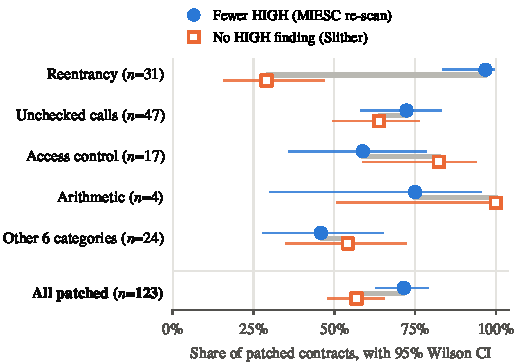
\includegraphics[width=\columnwidth]{figs/fig_validators}
\caption{Self-validation versus independent validation by category. Blue: share of patched contracts for which the MIESC re-scan reports fewer HIGH/CRITICAL findings. Orange: share with no HIGH finding under Slither. All 123 patches compile. The two metrics diverge most for reentrancy (30/31 vs.\ 9/31) because pre-existing HIGH findings from other detectors remain (Table~\ref{tab:prepost}). Circles and squares distinguish the series in greyscale.}
\label{fig:validators}
\end{figure}

Fig.~\ref{fig:validators} breaks the results down by category. The two metrics answer different questions and can diverge sharply. For reentrancy, the MIESC re-scan reports fewer HIGH findings for 30 of 31 patched contracts, yet only 9 are free of every HIGH finding under Slither. The pre-patch baseline (Table~\ref{tab:prepost}) explains the gap. Slither's own reentrancy detector fires on 28 of 29 analyzable reentrancy contracts before patching and on none afterwards; its 3 remaining reentrancy alerts belong to contracts of other categories. The HIGH alerts left on reentrancy contracts come from other detectors and were already present in the original code. Across all analyzable patched contracts, HIGH contract--detector pairs fall from 141 to 60, and the contracts free of HIGH findings rise from 35 to 69; 34 contracts become clean and none becomes non-clean (exact McNemar $p=1.2\times10^{-10}$). In 50 of the 52 contracts that stay non-clean, every remaining HIGH detector predates the patch. Two patches introduce a new HIGH alert (\texttt{arbitrary-send-eth} in one contract, \texttt{shadowing-state} in another), which we count as regressions under independent validation. The divergence also runs the other way: for access control, Slither finds more contracts clean (14/17) than the re-scan credits (10/17). Arithmetic has only 4 patched contracts because 11 of the 15 arithmetic contracts produce no current HIGH/CRITICAL finding, and the no-regression criterion fails only for 2 reentrancy contracts.

\begin{table}[htbp]
\caption{Slither HIGH Detectors Before and After Patching (number of contracts flagged; 121 analyzable patched contracts)}
\label{tab:prepost}
\centering
\footnotesize
\begin{tabular}{@{}lrr@{}}
\toprule
\textbf{Slither detector} & \textbf{Before} & \textbf{After} \\
\midrule
\texttt{reentrancy-eth} & 33 & 3 \\
\texttt{arbitrary-send-eth} & 29 & 2 \\
\texttt{msg-value-in-nonpayable} & 9 & 0 \\
\texttt{controlled-array-length} & 34 & 28 \\
\texttt{weak-prng} & 13 & 13 \\
\texttt{shadowing-state} & 8 & 9 \\
Other 6 detectors & 15 & 5 \\
\midrule
Contract--detector pairs & 141 & 60 \\
Contracts free of HIGH findings & 35 & 69 \\
\bottomrule
\end{tabular}

\vspace{2pt}
\scriptsize{Before: original contract, Slither 0.11.6; a detector counts if any of ten runs reports it (\texttt{encode-packed-collision} fired intermittently on one contract). After: canonical v2 external validation of the patched contract (single run). Script and per-contract results are released.}
\end{table}

\textbf{Experiment validity audit.} To separate patch quality from corpus compilability, we additionally compile the original contracts under the same standalone criterion. In the v2 run, 142/143 original files compile standalone. The patcher emits 123 patched contracts; all 123 compile, and all 123 are also checked by external Slither validation without tool errors.

\subsection{Stage 3: Test Validity}

\begin{table}[htbp]
\caption{Generated Foundry Tests (illustrative contract, $n$\,=\,1)}
\label{tab:tests}
\centering
\begin{tabular}{@{}lccc@{}}
\toprule
\textbf{Test} & \textbf{Compile} & \textbf{Vuln.} & \textbf{Fixed} \\
\midrule
Reentrancy (ETH) & \checkmark & Reverts\textsuperscript{a} & PASS \\
Reentrancy (cross-fn) & \checkmark & Reverts\textsuperscript{a} & PASS \\
Selfdestruct (unprotected) & \checkmark & Confirms\textsuperscript{b} & PASS \\
Selfdestruct (identifier) & \checkmark & Confirms\textsuperscript{b} & PASS \\
Unchecked return value & \checkmark & PASS & PASS \\
Uninitialized state & \checkmark & PASS & PASS \\
\midrule
\textbf{Total} & 6/6 & 2/6 discriminate & 6/6 \\
\bottomrule
\end{tabular}

\vspace{2pt}
\footnotesize{Vuln.: exploit-confirmation test on the vulnerable contract. Fixed: fixed-version regression test on the patched contract. \textsuperscript{a}The re-entrant call reverts with an arithmetic underflow (Solidity 0.8 checked arithmetic); the patched contract also reverts, at the guard, so these tests do not discriminate. \textsuperscript{b}The test expects a revert for a non-owner caller; the call succeeds on the vulnerable contract and reverts on the patched one.}
\end{table}

The scan of the illustrative contract yields one test per supported finding, including two findings (unchecked return value, uninitialized state) beyond its five intentional vulnerabilities; the missing-access-control finding is covered by the two selfdestruct tests, which exercise the same unprotected functions. All 6 tests compile with Foundry, and all 6 fixed-version regression tests pass on the patched contract. Only the two selfdestruct tests behave differently on the vulnerable and the patched contract. The two reentrancy tests revert on both versions under Solidity~0.8 (see below), and the other two pass on both, so 4 of the 6 tests do not discriminate between vulnerable and patched code.

\textbf{Reentrancy exploit test.} Listing~\ref{lst:exploit} shows the Foundry test generated by \texttt{miesc test-gen} for the reentrancy finding. The test deploys an attacker contract that re-enters \texttt{withdraw()} from its \texttt{receive()} fallback and asserts that the attacker ends with more than its deposit. Under Solidity~0.8 checked arithmetic, the nested balance decrements underflow and the whole call reverts, so the assertion is never reached; with the inline guard, the first re-entrant call reverts instead. On 0.8 code the test therefore does not observe a drain on either version.

\begin{lstlisting}[caption={Generated exploit test for reentrancy (simplified)},label={lst:exploit},float=htbp]
contract Attacker {
    Vault target;
    uint256 count;

    constructor(address _target) {
        target = Vault(_target);
    }

    function attack() external payable {
        target.deposit{value: 1 ether}();
        target.withdraw(1 ether);
    }

    receive() external payable {
        if (count < 5) {
            count++;
            target.withdraw(1 ether);
        }
    }
}

contract ReentrancyTest is Test {
    function test_drain() public {
        Vault vault = new Vault();
        vm.deal(address(vault), 6 ether);
        Attacker atk = new Attacker(
            address(vault));
        vm.deal(address(atk), 1 ether);
        vm.prank(address(atk));
        atk.attack();
        assertGt(address(atk).balance, 1 ether);
    }
}
\end{lstlisting}

A discriminating reentrancy test for 0.8 code would have to compare outcomes (e.g., expect the drain on the vulnerable contract and a revert on the patched one), or target code whose decrement is unchecked; generating such tests is part of our future work. For each supported category, \texttt{test-gen} also emits a fixed-version regression test that expects the exercised path to be blocked after patching.

\subsection{Stage 4: Formal Verification}

The formal verification stage applies the Solidity compiler's built-in SMTChecker using the Constrained Horn Clauses (CHC) engine~\cite{solidity_smtchecker}. Unlike fuzzers that generate concrete test inputs, CHC-based verification checks encoded properties over symbolic execution paths via fixed-point computation over the contract's control-flow graph.

\textbf{Methodology.} For each finding, \texttt{miesc specs} generates one or more \texttt{assert()} statements encoding the property that should hold after patching. The SMTChecker is invoked with \texttt{-{}-model-checker-engine chc} and \texttt{-{}-model-checker-targets assert,underflow,overflow}. We compare warnings between the original and patched contracts.

\textbf{Results on illustrative contract.} The vulnerable \texttt{AuditTarget.sol} produces 2 SMTChecker warnings and 1 compiler warning:
\begin{itemize}
    \item \textbf{Underflow} at line 42 (\texttt{balances[msg.sender] -= amount}): reachable when \texttt{amount > balances[msg.sender]} after re-entry modifies the balance.
    \item \textbf{Assertion violation} on the generated \texttt{assert(address(this).balance >= sum\_of\_balances)} invariant: violated because re-entry drains more than the sender's legitimate balance.
    \item \textbf{Unchecked low-level call} (compiler warning, not an SMTChecker target): the return value of \texttt{.call} is not used.
\end{itemize}

After patching, the first two warnings disappear entirely (the reentrancy guard makes the re-entry path unreachable), and the third is resolved by the \texttt{require(success)} wrapper. On this tractable example, CHC verification provides stronger evidence than the exploit test because it checks the encoded assertion over symbolic executions rather than over one concrete exploit trace.

\textbf{Why no corpus-wide CHC figure.} The CHC engine is driven through the \texttt{-{}-model-checker-engine} options of recent compilers (we use 0.8.20); the 0.4.24--0.5.17 compilers that the corpus requires do not offer them, and 142 of the 143 SmartBugs contracts declare a 0.4.x pragma. A corpus-wide CHC measurement would therefore first require porting the contracts to 0.8, which would change the code under test. The evidence for Contribution~3 is limited to the illustrative contract, and a CHC evaluation on a modern 0.8 corpus is future work. This limitation motivates the hybrid approach: exploit tests provide fast executable evidence, while formal verification adds stronger assurance only when the generated specification is tractable.

\subsection{Stage 5: Compliance and Reporting}

The compliance mapper assigns each finding to applicable controls using a rule-based mapper with 12 standard and taxonomy profiles. On the illustrative contract, the mapper's rules assign 4 of 11 findings to MiCA, 3 to the NIST CSF~1.1 access-control category PR.AC-4, and 2 to ISO~27001:2022 control A.8.26 (application security requirements). These assignments follow the tool's rule set and are not a legal assessment of regulatory scope. The report generator produces a 3{,}060-line HTML premium audit report with proof-of-concept (PoC) templates, Common Vulnerability Scoring System (CVSS) v3.1 estimates (base score computation from finding severity and attack vector), and a prioritized remediation roadmap.

\subsection{End-to-End Pipeline (Illustrative)}
\label{sec:e2e}

On the illustrative contract, the scan reports 11 findings (1 critical, 4 high, 4 medium, 2 low). The patcher applies 3 patches (2 further findings are deduplicated onto the same functions), and no HIGH-severity finding remains on re-scan. The 6 generated tests all compile (Table~\ref{tab:tests} details their limits), one SMTChecker specification is generated, 4 findings map to MiCA, and a 3{,}060-line HTML report is produced. The complete run takes under 10 seconds in local mode with no API cost. These per-stage counts describe one contract and carry no statistical weight; the corpus-scale evidence is in Table~\ref{tab:fix} and Fig.~\ref{fig:validators}.

\subsection{Comparison with Prior Work}
\label{sec:comparison}

\begin{table}[htbp]
\caption{Feature comparison with prior repair tools. T/S/C~= generates exploit tests / formal specs / compliance mapping.}
\label{tab:comparison}
\centering
\scriptsize
\setlength{\tabcolsep}{3pt}
\begin{tabular}{@{}lcccccc@{}}
\toprule
\textbf{Tool} & \textbf{Yr} & \textbf{Vulns} & \textbf{Fix\%} & \textbf{Comp.\%} & \textbf{T} & \textbf{S/C} \\
\midrule
SCRepair~\cite{screpair2020} & '20 & GP & --- & --- & Req\textsuperscript{a} & \texttimes/\texttimes \\
sGuard~\cite{nguyen2021sguard} & '21 & 4 & --- & ${\sim}$100 & \texttimes & \texttimes/\texttimes \\
Elysium~\cite{elysium2022} & '22 & 7 SWC & +30\textsuperscript{b} & --- & \texttimes & \texttimes/\texttimes \\
ACFIX~\cite{acfix2024} & '25 & 1 & 94.9 & --- & \texttimes & \texttimes/\texttimes \\
SCPatcher~\cite{scpatcher2025} & '26 & Gen. & 81.5 & 91 & \texttimes & \texttimes/\texttimes \\
\textbf{MIESC} & '26 & 4 fix cl.\textsuperscript{d} & 72\textsuperscript{c} & 100 & \checkmark & \checkmark/\checkmark \\
\bottomrule
\end{tabular}

\vspace{2pt}
\scriptsize{GP: genetic programming. \textsuperscript{a}Requires pre-existing test suite. \textsuperscript{b}More contracts correctly patched than existing tools. \textsuperscript{c}Each tool's own definition and scope; for MIESC, HIGH/CRITICAL count reduced on re-scan. Not directly comparable; shown for context, not ranking. \textsuperscript{d}Four template classes applied across the 10 corpus categories.}
\end{table}

Table~\ref{tab:comparison} compares MIESC against five prior automated repair tools. MIESC reaches 100\% standalone compilation for emitted patches (123/123) under a strict no-external-dependency criterion, while SCPatcher reports 91\% compilation under different evaluation targets and dependency assumptions, so the numbers are not directly interchangeable; the MIESC ``Fix\%'' column reports the share of patched contracts with fewer HIGH/CRITICAL findings on re-scan (88/123, 72\%). ACFIX reports 94.9\% fix rate but is limited to a single vulnerability class (RBAC). Of the five compared tools, MIESC is the only one that emits artifacts across the remediation lifecycle (patch generation, exploit testing, formal specifications, and compliance mapping), with the latter three demonstrated on one contract.

\subsection{Failure Analysis}

In the v2 baseline, standalone compilation is no longer a failure mode: all 123 emitted patches compile (versus 51/141 failures in v1; see Section~\ref{sec:setup}). The remaining v2 gaps are therefore semantic rather than syntactic: 35/123 patched contracts show no reduction in HIGH/CRITICAL findings on MIESC re-scan, and external Slither validation finds only 70/123 patched contracts clean of HIGH (57\%), with 53 contracts still reporting HIGH findings.

This reframes the root-cause direction for future work. With standalone compilation solved, the priority shifts from symbol-resolution repair to semantic adequacy: removing the targeted flaw without introducing new HIGH findings under independent validation. The external-validation gap (53 contracts with residual HIGH findings; in 50 of the 52 analyzable ones every remaining detector predates the patch) points to the main lever: extending the templates to \texttt{controlled-array-length}, \texttt{weak-prng} and \texttt{shadowing-state}.

% ===========================================================================
\section{Discussion}
% ===========================================================================

\subsection{Limitations of Text-Level Patching}\label{sec:textlevel}

MIESC's patcher operates at the text level rather than on the abstract syntax tree (AST). This design choice favors portability (no AST tooling or compiler-specific front end is required) at the cost of precision. Specifically:

\begin{enumerate}
    \item \textbf{No code restructuring}: the patcher cannot reorder statements to implement the Checks-Effects-Interactions (CEI) pattern---the gold standard for reentrancy prevention. Instead, it adds a mutex guard, which is a conservative mitigation but stylistically different from what a human auditor would write.
    \item \textbf{Regex-based function matching}: unusual formatting (multi-line signatures, Unicode comments, inline assembly, or comments that contain code) can cause mismatched insertions. In the v2 run this risk did not appear as standalone compilation failure for emitted patches, but it remains a design risk for repositories with more complex formatting and dependencies.
    \item \textbf{Single-contract scope}: cross-contract vulnerabilities (e.g., a proxy's \texttt{delegatecall} to a malicious implementation) cannot be patched because the fix requires coordinating changes across multiple files.
\end{enumerate}

These limitations define the tradeoff behind the design. Text-level patching gives broad current-scan coverage across the corpus compilers (0.4.24--0.5.17) and, in the v2 run, 100\% standalone compilation for emitted patches. AST-level approaches like sGuard can be more precise, but they usually depend on narrower compiler and AST assumptions.

\subsection{Test Coverage and Correctness}

The generated tests cover the \emph{specific vulnerability} reported by the scanner, not general contract behavior. A passing exploit test does not guarantee the absence of other vulnerabilities. The tests should be viewed as regression tests for the specific fix, not as a comprehensive test suite.

Importantly, the exploit tests serve a dual role: (1)~when they discriminate, they provide executable evidence for the detection (a test that cannot trigger the vulnerability is a prompt to re-examine the finding, although, as the reentrancy case shows, a real flaw may also be untriggerable under 0.8 checked arithmetic), and (2)~they check the patched path exercised by the exploit (if the same exploit still succeeds after patching, the fix is incomplete). None of the repair tools in our comparison reports this kind of bidirectional check.

\subsection{Cost}

The evaluated patcher is rule-based and runs locally with no API cost. LLM providers enter only through the detection stage, where local models avoid API costs and frontier providers can be reserved for disputed HIGH/CRITICAL findings. Automated patches are suggestions for review, not changes to merge unreviewed.

\subsection{Towards Continuous Security}

The illustrative pipeline's sub-10-second execution time suggests a practical CI/CD integration pattern. A GitHub Action running \texttt{miesc scan -{}-ci} on every pull request, combined with \texttt{miesc fix -{}-dry-run} to suggest patches in PR comments, would provide continuous security feedback without blocking development velocity. This integration pattern---detection as a gate, remediation as a suggestion---preserves developer autonomy while making security findings visible earlier in the development process.

\subsection{Threats to Validity}
\label{sec:threats}

We group seven threats to validity into four categories:

\textbf{Internal validity.} (1)~\emph{Scan non-determinism}: the detection scans that feed the patcher come from the companion paper's reproducible profile and are stored as artifacts; 2 scans were retried after empty output, and re-running them may yield slightly different findings. (2)~\emph{Re-scan verification}: the fewer-HIGH criterion is measured by re-scanning the patched contract with the same pipeline family that detected the original vulnerability, so a false negative on re-scan would inflate that rate. The v2 baseline mitigates this by adding external Slither validation over every patched contract that compiles and a pre-patch Slither baseline, reporting both separately from the MIESC re-scan rather than merging them into a single success metric. Slither also contributes to MIESC's own static layer, so this validation is external to the re-scan rather than fully independent of the detection pipeline; the before/after comparison is still informative because the patcher never edits code to silence a detector. For reentrancy, Slither's own detector flags 28 of 29 analyzable contracts before patching and none after.

\textbf{External validity.} (3)~\emph{Corpus selection bias}: SmartBugs-curated consists mostly of small legacy contracts with known vulnerabilities (142 of 143 declare a 0.4.x compiler pragma). These contracts are small (85 non-blank lines on average, computed over the corpus) and heavily studied, whereas production decentralized-finance (DeFi) protocols are typically larger, multi-file and deeply inherited. Results on production code may differ, particularly for the compilation rate (which depends heavily on dependency availability). (4)~\emph{Vulnerability distribution}: the corpus over-represents reentrancy (31 contracts) and unchecked low-level calls (52 contracts) relative to their frequency in production code. Categories such as oracle manipulation, maximal extractable value (MEV) and flash-loan attacks, which account for many recent DeFi incidents~\cite{zhou2023sok}, are absent from SmartBugs.

\textbf{Construct validity.} (5)~\emph{Compilation $\neq$ correctness}: a compiling patch is not necessarily semantically correct. The patch could introduce subtle behavioral changes (e.g., a reentrancy guard that blocks legitimate callback patterns). Our no-regression criterion measures only re-scan finding growth under the same pipeline, and the external Slither clean-HIGH metric measures only residual HIGH findings under one independent analyzer; neither proves preservation of all original functional behavior. (6)~\emph{Artifact granularity}: test generation, formal verification, and compliance reporting are evaluated end-to-end on an illustrative contract, while patch quality is measured corpus-wide. We therefore do not claim corpus-wide proof coverage for all generated artifacts.

\textbf{Development-set overlap.} (7)~\emph{No held-out set}: the patch templates (reentrancy guard, access-control modifier, checked-call rewrite, SafeMath directive) were developed against SmartBugs-curated itself; the evaluation corpus therefore doubles as the development corpus, with no held-out test split. The reported patch-quality rates should be read as in-distribution results. The transforms are standard, category-level rewrites rather than per-contract fixes---and we explicitly avoid detector-silencing edits---but generalization to unseen contracts is not measured here and remains future work.

\textbf{Residual threats.} Threats (3) and (4) are not mitigated for the remediation stage. Our companion paper~\cite{boiero2025miesc} evaluates detection on business-logic vulnerabilities from real audits, but remediation on modern production contracts remains future work.

% ===========================================================================
\section{Conclusion and Future Work}
% ===========================================================================

This paper reports how far the current MIESC remediation pipeline can move after detection, and where it still falls short. On 143 SmartBugs-curated contracts, the v2 baseline patches 123, and all 123 patches compile standalone. The MIESC re-scan reports fewer HIGH/CRITICAL findings for 88 of them, and 121 satisfy the bounded no-regression criterion. Under independent Slither validation, 70 are free of HIGH findings (57\%; 95\% CI [48\%, 65\%]); on the 121 contracts with a pre-patch baseline, that count rises from 35 to 69, and Slither's reentrancy detector, which flags 28 of 29 analyzable reentrancy contracts before patching, flags none afterwards. Reporting the external metric separately shows that patch emission and compilation do not imply semantic closure. Among the five prior repair tools we compare (Table~\ref{tab:comparison}), MIESC is the only one that reports exploit tests, formal specifications, and compliance documentation alongside patches.

The design choice is to keep each stage inspectable. Detection informs patching, patching informs test generation, test generation checks the exercised exploit path, and formal verification can add stronger evidence when the generated specification is tractable. The current evidence supports this as a workflow that automates the generation of repair candidates for human review, not as a claim of correct automatic program repair.

\textbf{Limitations.} The 100\% standalone compilation rate applies to emitted patches after current-scan filtering. Test generation, specification generation, and compliance mapping are demonstrated on a single contract, and the generated reentrancy tests do not discriminate on 0.8 code; Sections~\ref{sec:textlevel} and~\ref{sec:threats} discuss the remaining limitations.

\textbf{Future work.} Three directions are planned: (1)~\emph{AST-level patching} via Slither's intermediate representation, enabling CEI reordering, cross-contract fixes and templates for the residual detector classes; (2)~\emph{corpus-scale evaluation of tests, specifications and compliance mapping} on a modern 0.8 corpus, with discriminating exploit tests and CHC discharge rates; and (3)~\emph{production-scale evaluation} on multi-file DeFi protocols with dependency-aware compilation.

MIESC, the evaluation scripts, and the per-claim artifacts are available under AGPL-3.0 at \url{https://github.com/fboiero/MIESC}.

% ===========================================================================
\section*{Acknowledgment}
% ===========================================================================

This work continues research at Universidad Tecnol\'ogica Nacional, Facultad Regional Villa Mar\'ia (UTN-FRVM). The authors thank the Ethereum security community and the developers of Foundry, Slither, and OpenZeppelin.

\bibliographystyle{IEEEtran}
\bibliography{references}

\end{document}
